\section{Résultats et interprétations}

Nous avons fait tourner cette simulation pour une durée totale physique de 26141802 secondes, soit l'équivalent de 302.6 jours. 
Les solutions pour chaque $r$ de la branche supérieure déterminées par dichotomie ne sont pas équivalentes aux branches atteintes dans la simulation. Nous pouvons voir sur la figure (\ref{fig:qmap}) en rouge la branche déterminée par dichotomie correspondant à $\tau_{ff} = 0.06 $ et en blanc celle correspondant à la valeur théorique $\tau_{ff} = 1$. Les possibles raisons de ces écarts sont dévelopés partie (\ref{sec::pistes}). La simulation est bien en accord avec le passage d'un disque optiquement épais à un disque optiquement mince. Nous pouvons voir figure (\ref{fig:c1.eps}) et (\ref{fig:c20.eps}) comment se comporte le système du point de vue de ces deux grandeurs physiques. \FIXME{parler de l'instabilité} \\
 

\begin{figure}
  \begin{center}
    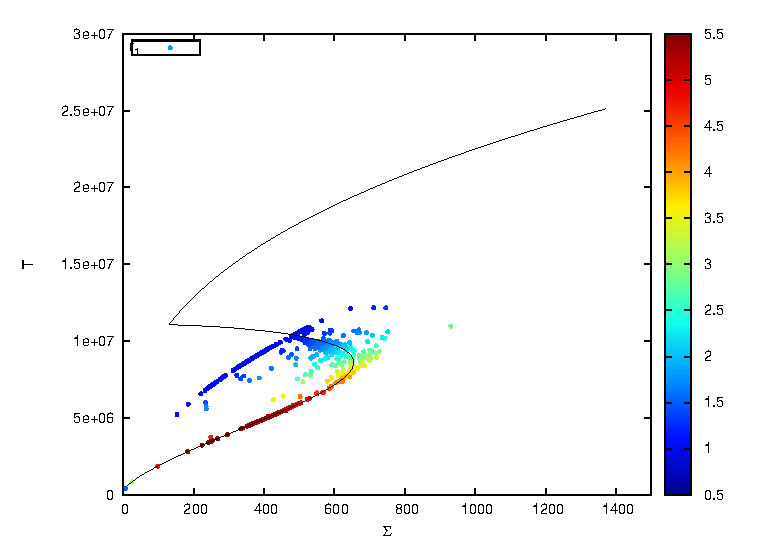
\includegraphics[]{c1.eps}
  \end{center}
  \caption{$T=f(\Sigma)$, $\Delta t = 26141802 s$ (durée de la simulation) pour $r_{1}$. Le gradiant de couleur représente les valeurs de $\tau_{ff}$}
  \label{fig:c1.eps}
\end{figure} 

\begin{figure}
  \begin{center}
    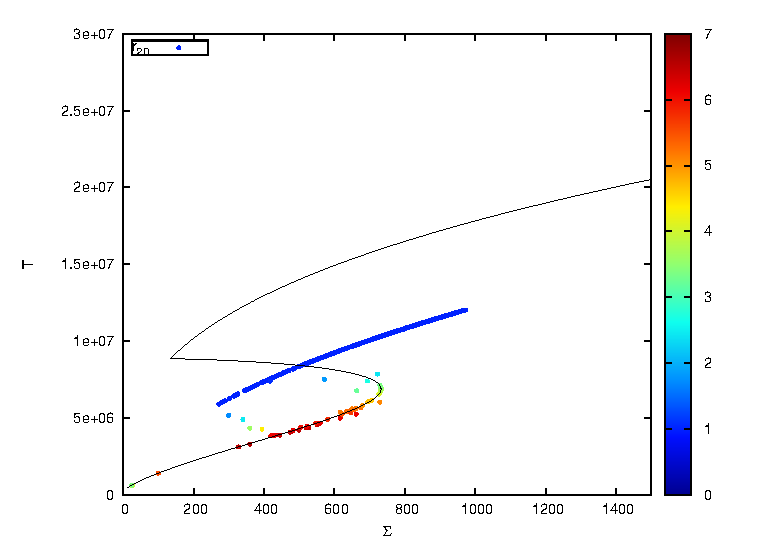
\includegraphics[]{c20.eps}
  \end{center}
  \caption{$T=f(\Sigma)$, $\Delta t = 26141802 s$ (durée de la simulation) pour $r_{20}$. Le gradiant de couleur représente les valeurs de $\tau_{ff}$}
  \label{fig:c20.eps}
\end{figure}


